\documentclass[12pt]{article}
\usepackage[spanish]{babel}
\usepackage{geometry}
\geometry{a4paper, margin=1in}
\usepackage{graphicx}
\usepackage{xcolor}
\usepackage{titlesec}
\usepackage{parskip}
\usepackage{multicol}
\usepackage{cite}

\definecolor{highlight}{RGB}{255, 255, 0}

\titleformat{\section}{\normalfont\Large\bfseries}{\thesection}{1em}{}
\titleformat{\subsection}{\normalfont\large\bfseries}{\thesubsection}{1em}{}

\begin{document}

% Logos
\begin{minipage}{0.45\textwidth}
    
\includegraphics[width=0.4\textwidth]{inFiles/Figures/epnLogo.jpg}
\end{minipage}
\hfill
\begin{minipage}{0.45\textwidth}
    \raggedleft
    
\includegraphics[width=0.4\textwidth]{inFiles/Figures/FIS_logo.jpg}
\end{minipage}

\vspace{0.5cm}

% Títulos principales
\begin{center}
    \textbf{ESCUELA POLITÉCNICA NACIONAL}\\[0.2cm]
    \textbf{FACULTAD DE INGENIERÍA DE SISTEMAS}\\[0.2cm]
    \textbf{INGENIERÍA {\textbf{EN COMPUTACION}}}
\end{center}

\vspace{0.5cm}
\hrule
\vspace{0.5cm}

% Datos principales
\noindent\textbf{PERÍODO ACADÉMICO:} 2025-A\\[0.2cm]    
\noindent\textbf{ASIGNATURA:} ICCD412 Métodos Numéricos \hfill \textbf{GRUPO:} GR2\\[0.2cm]
\noindent\textbf{TIPO DE INSTRUMENTO:} {Deber N°7}\\[0.2cm]
\noindent\textbf{FECHA DE ENTREGA LÍMITE:} {09/05/2025}\\[0.2cm]
\noindent\textbf{ALUMNO:} {Lema Luis}

\vspace{0.5cm}
\hrule
\vspace{1cm}


% Secciones
\section*{TEMA}
{Método de Newton, Secante y Posición Falsa}

\vspace{0.5cm}

\section*{OBJETIVOS}
\begin{itemize}
    \item { Aplicar lo aprendido en clase para desarrollar los ejercicios propuestos}

\end{itemize}

\vspace{0.5cm}

\section*{DESARROLLO}


\begin{minipage}{0.95\textwidth}
    \raggedleft
    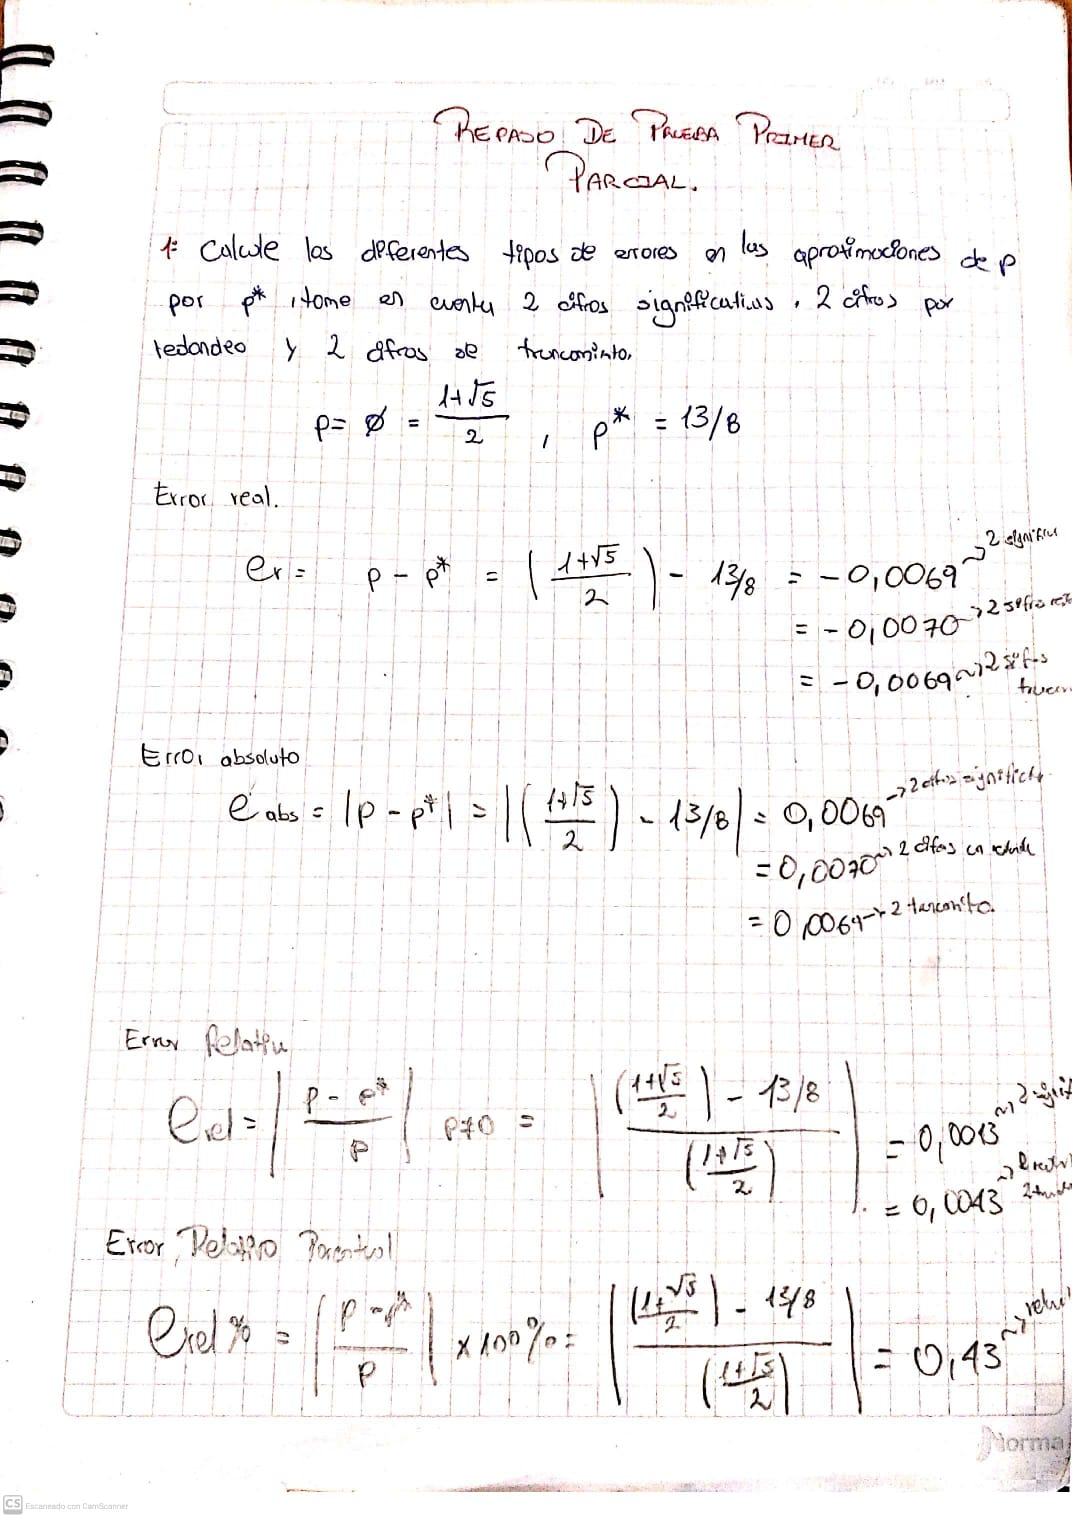
\includegraphics[width=1.15\textwidth]{inFiles/Figures/ejer1.jpeg}
\end{minipage}

\vspace{0.5cm}
\begin{itemize}

\begin{minipage}{0.95\textwidth}
    \raggedleft
    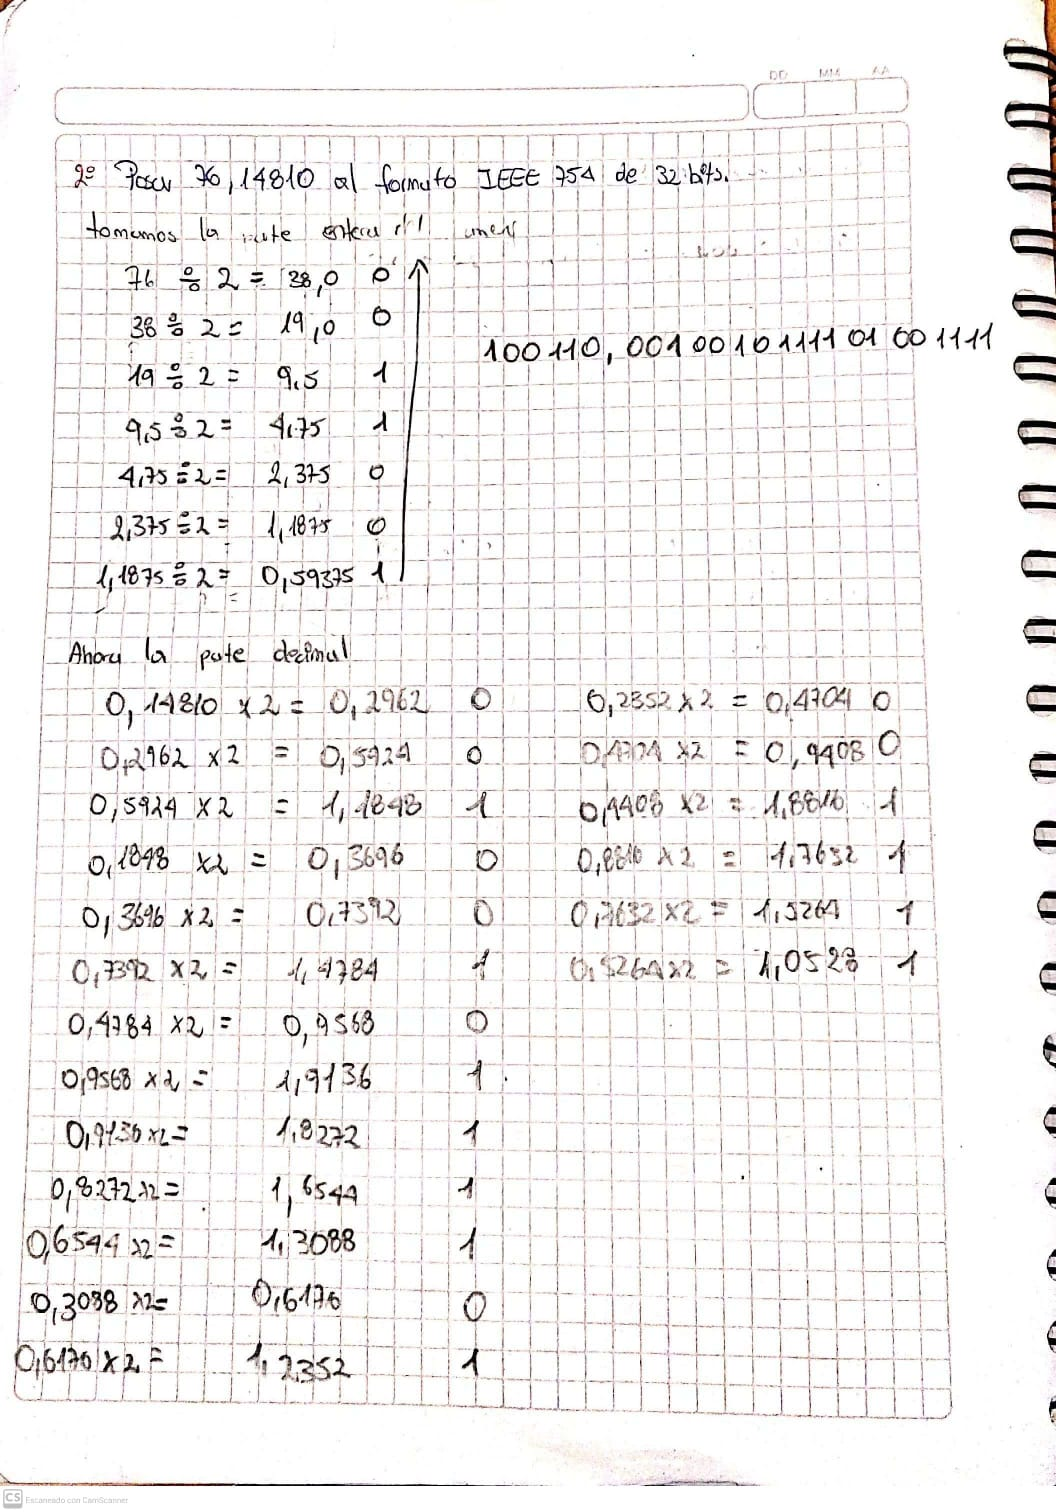
\includegraphics[width=1.15\textwidth]{inFiles/Figures/ejer2.jpeg}
\end{minipage}
\vspace{1.5cm}

\begin{minipage}{0.95\textwidth}
    \raggedleft
    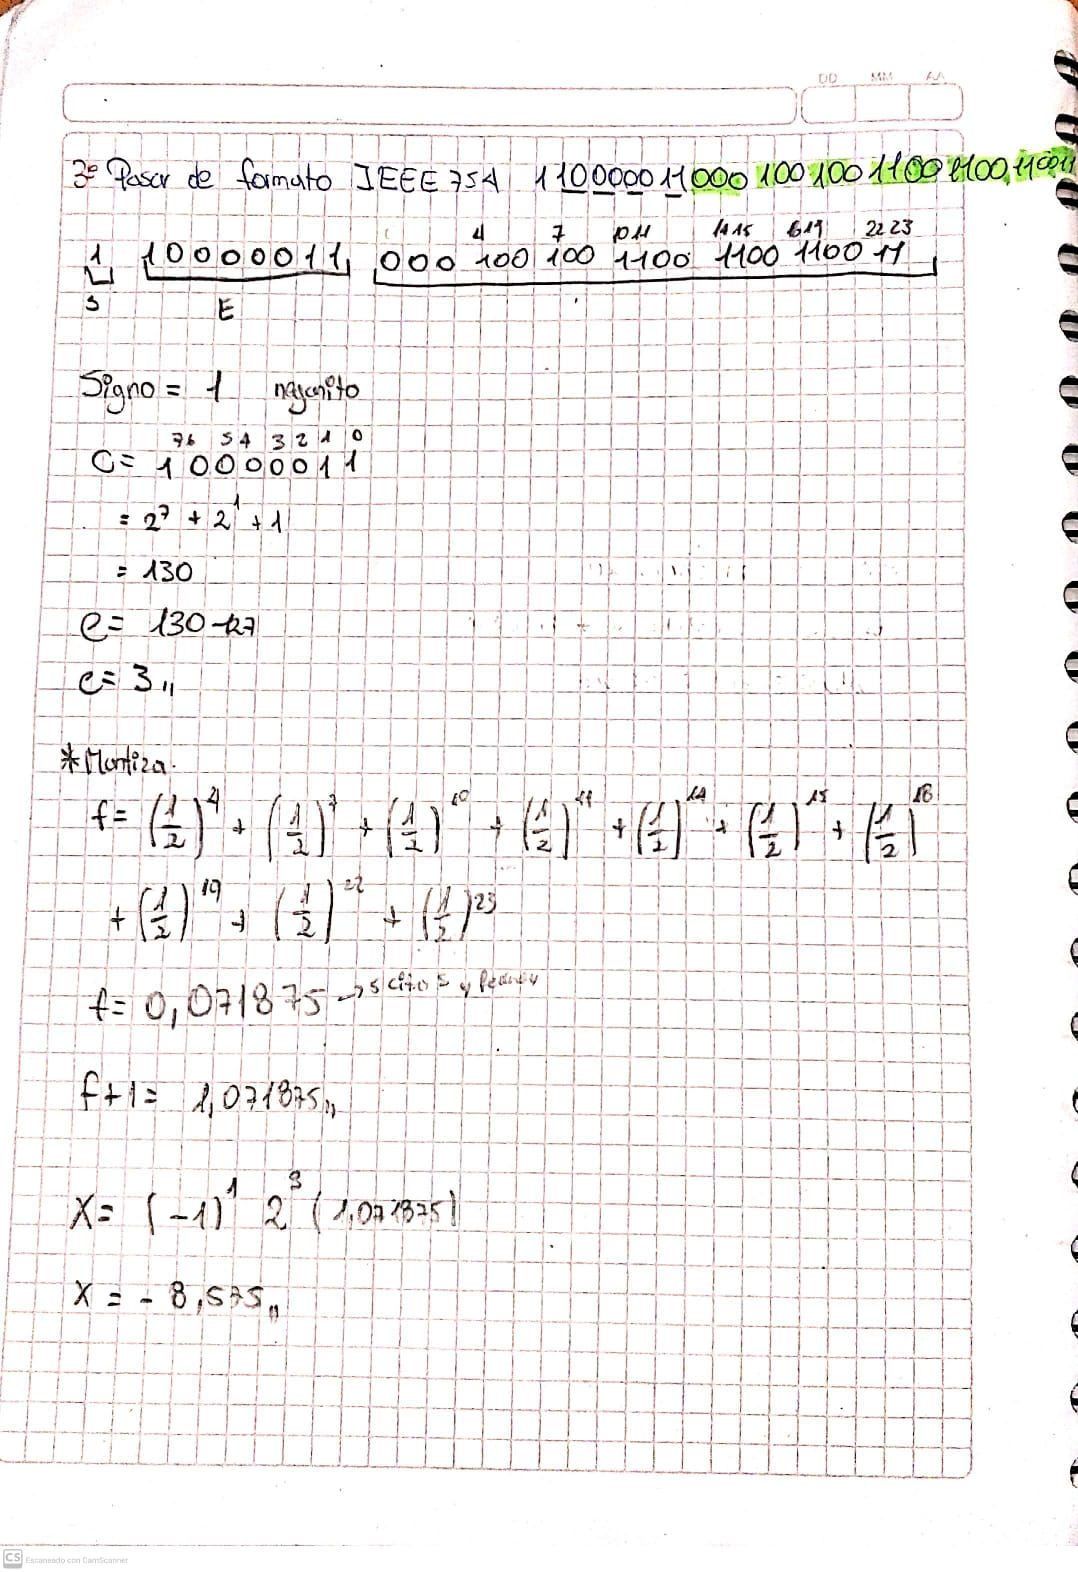
\includegraphics[width=1.15\textwidth]{inFiles/Figures/ejer3.jpeg}
\end{minipage}
\vspace{0.5cm}


\begin{minipage}{0.95\textwidth}
    \raggedleft
    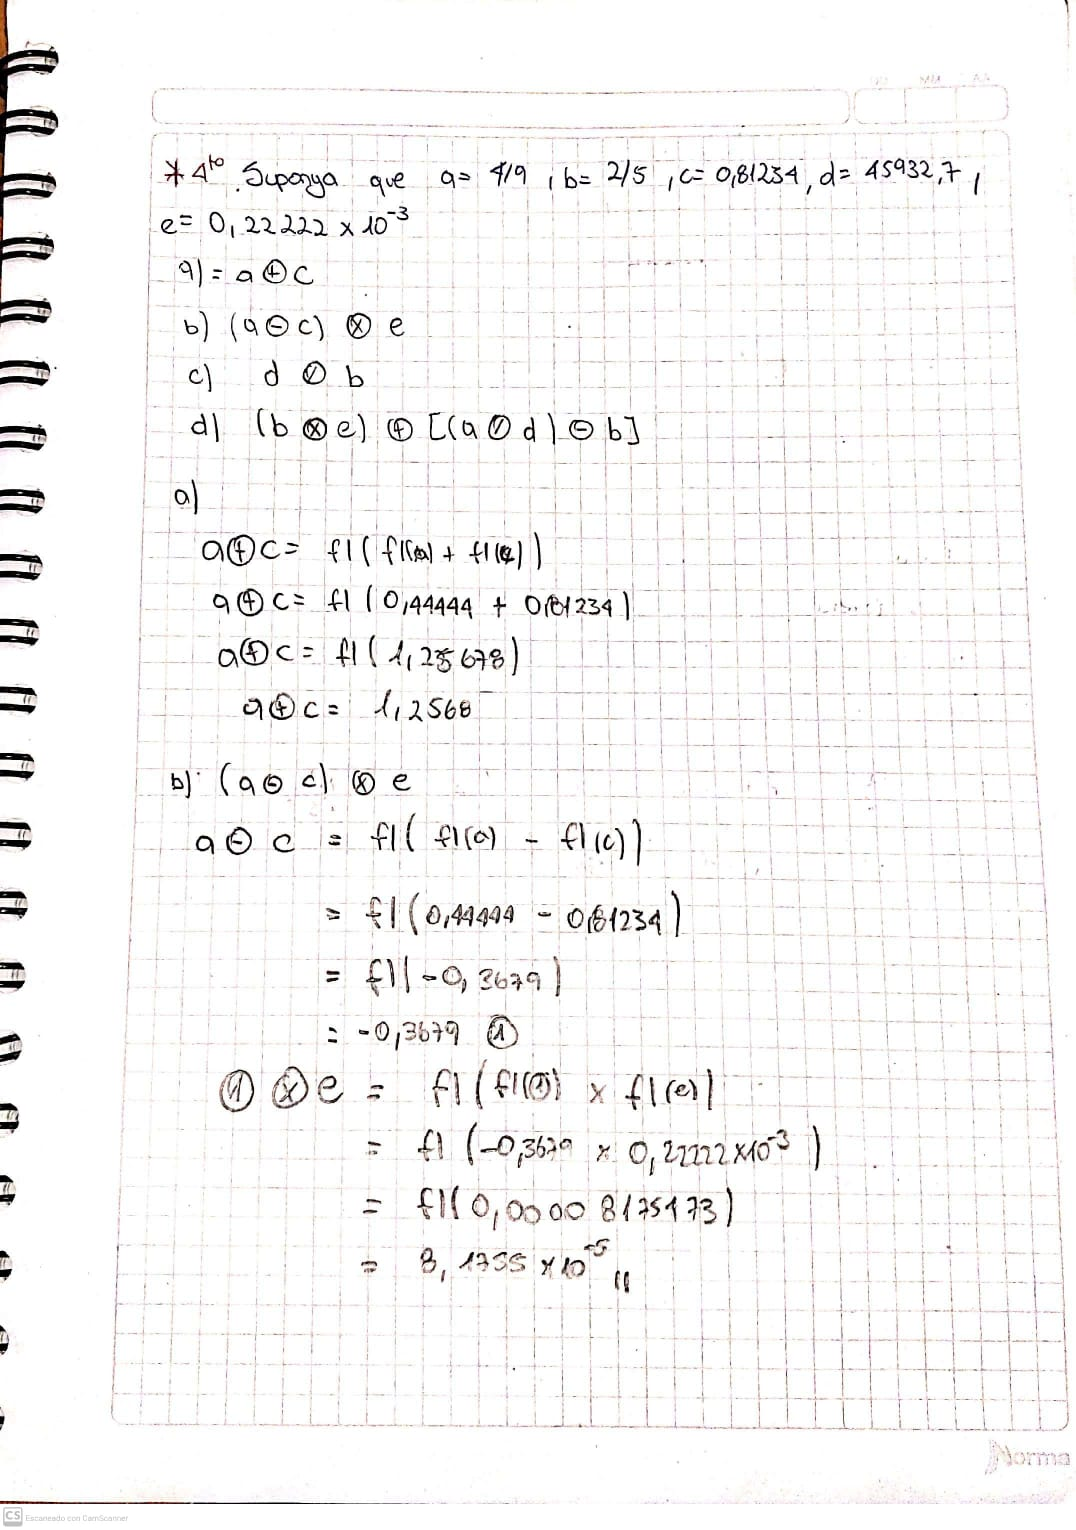
\includegraphics[width=1.15\textwidth]{inFiles/Figures/ejer4.jpeg}
\end{minipage}
\vspace{1.5cm}

\begin{minipage}{0.95\textwidth}
    \raggedleft
    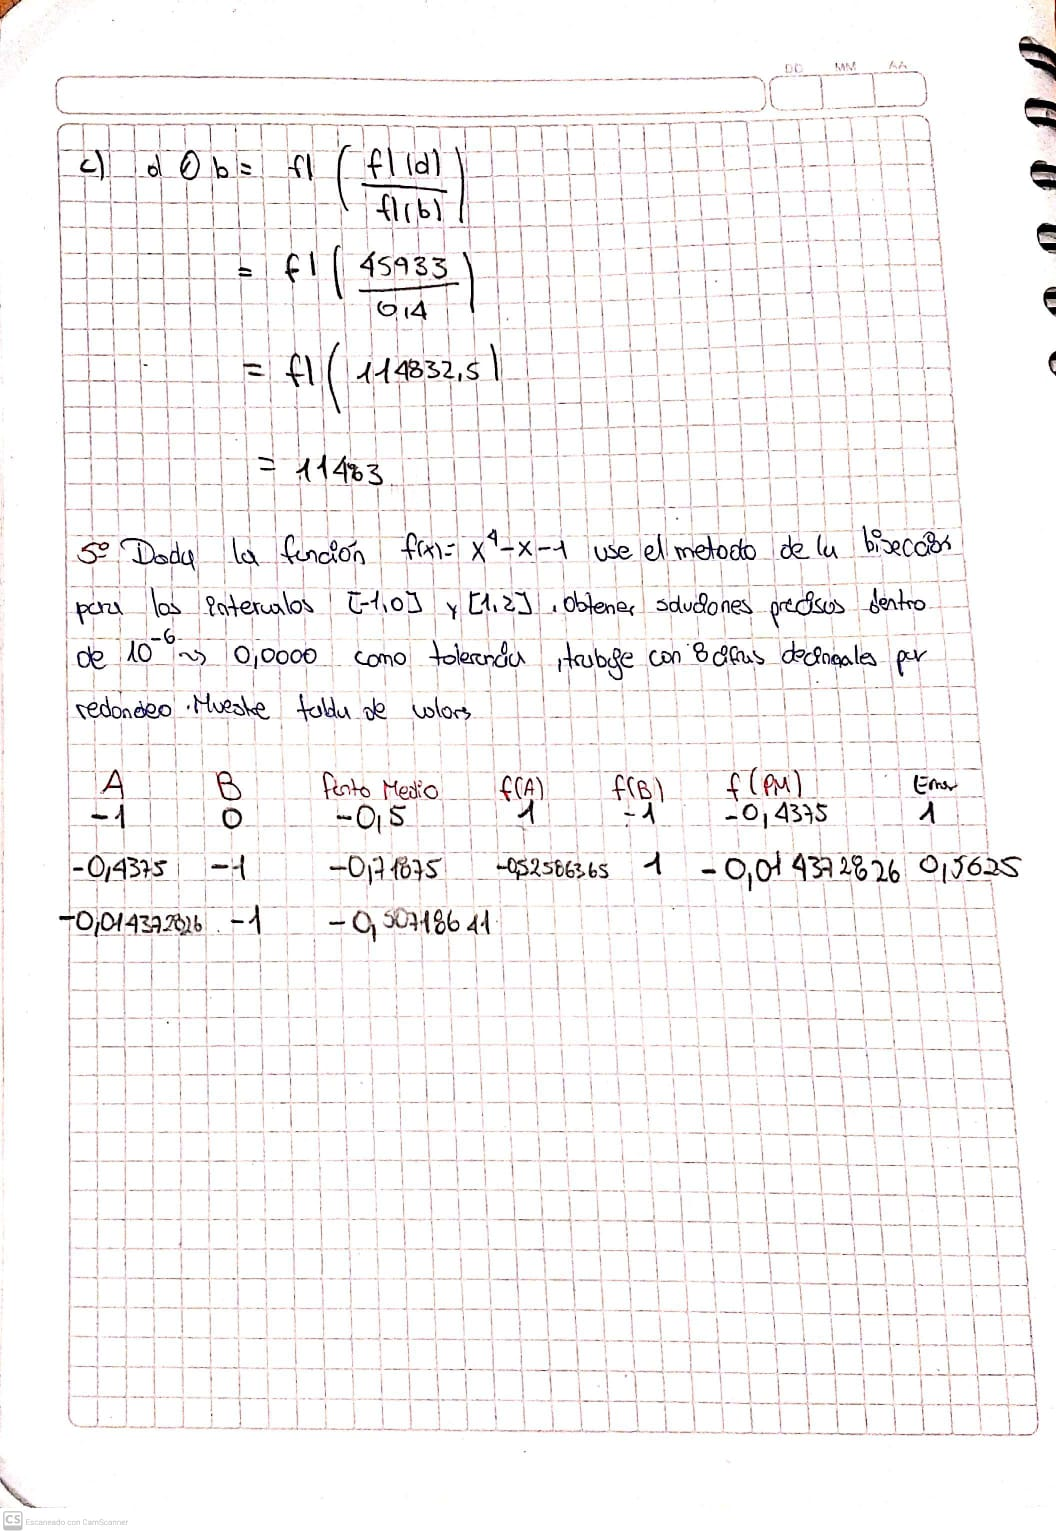
\includegraphics[width=1.15\textwidth]{inFiles/Figures/ejer5.jpeg}
\end{minipage}
\vspace{3.5cm}

\begin{minipage}{0.95\textwidth}
    \raggedleft
    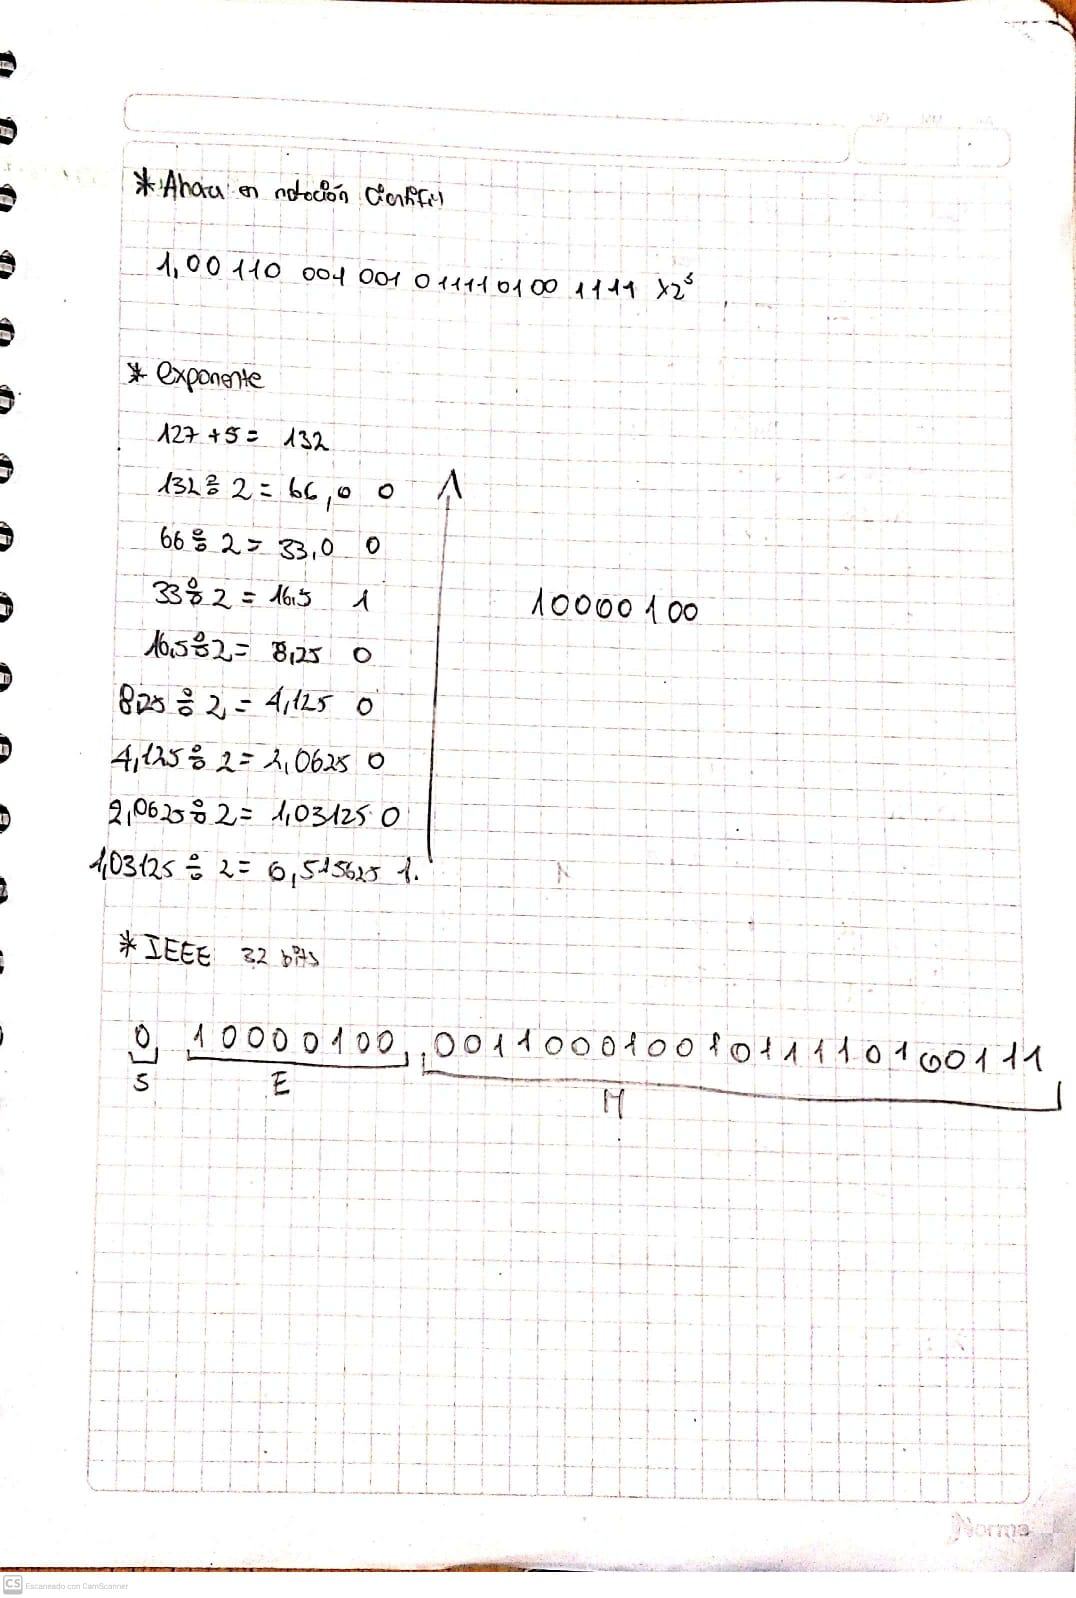
\includegraphics[width=1.15\textwidth]{inFiles/Figures/ejer6.jpeg}
\end{minipage}
\vspace{1.5cm}

\vspace{1.5cm}



\end{document}
